
%<<setup-child, include = FALSE>>=
%library(knitr)
%library(microbenchmark)
%library(reshape2)
%library(ggplot2)
%set_parent("../style/preamble.Rnw")
%
%set.seed(1)
%@

\input{../../2021/style/preamble4tex}
% dependencies: amsmath, amssymb, dsfont
% math spaces
\ifdefined\N
\renewcommand{\N}{\mathds{N}} % N, naturals
\else \newcommand{\N}{\mathds{N}} \fi
\newcommand{\Z}{\mathds{Z}} % Z, integers
\newcommand{\Q}{\mathds{Q}} % Q, rationals
\newcommand{\R}{\mathds{R}} % R, reals
\ifdefined\C
\renewcommand{\C}{\mathds{C}} % C, complex
\else \newcommand{\C}{\mathds{C}} \fi
\newcommand{\continuous}{\mathcal{C}} % C, space of continuous functions
\newcommand{\M}{\mathcal{M}} % machine numbers
\newcommand{\epsm}{\epsilon_m} % maximum error

% counting / finite sets
\newcommand{\setzo}{\{0, 1\}} % set 0, 1
\newcommand{\setmp}{\{-1, +1\}} % set -1, 1
\newcommand{\unitint}{[0, 1]} % unit interval

% basic math stuff
\newcommand{\xt}{\tilde x} % x tilde
\newcommand{\argmin}{\mathop{\mathrm{arg\,min}}} % argmin
\newcommand{\argmax}{\mathop{\mathrm{arg\,max}}} % argmax
\newcommand{\argminlim}{\argmin\limits} % argmin with limits
\newcommand{\argmaxlim}{\argmax\limits} % argmax with limits
\newcommand{\sign}{\operatorname{sign}} % sign, signum
\newcommand{\I}{\mathbb{I}} % I, indicator
\newcommand{\order}{\mathcal{O}} % O, order
\newcommand{\bigO}{\mathcal{O}} % Big-O Landau
\newcommand{\littleo}{{o}} % Little-o Landau
\newcommand{\pd}[2]{\frac{\partial{#1}}{\partial #2}} % partial derivative
\newcommand{\floorlr}[1]{\left\lfloor #1 \right\rfloor} % floor
\newcommand{\ceillr}[1]{\left\lceil #1 \right\rceil} % ceiling
\newcommand{\indep}{\perp \!\!\! \perp} % independence symbol

% sums and products
\newcommand{\sumin}{\sum\limits_{i=1}^n} % summation from i=1 to n
\newcommand{\sumim}{\sum\limits_{i=1}^m} % summation from i=1 to m
\newcommand{\sumjn}{\sum\limits_{j=1}^n} % summation from j=1 to p
\newcommand{\sumjp}{\sum\limits_{j=1}^p} % summation from j=1 to p
\newcommand{\sumik}{\sum\limits_{i=1}^k} % summation from i=1 to k
\newcommand{\sumkg}{\sum\limits_{k=1}^g} % summation from k=1 to g
\newcommand{\sumjg}{\sum\limits_{j=1}^g} % summation from j=1 to g
\newcommand{\summM}{\sum\limits_{m=1}^M} % summation from m=1 to M
\newcommand{\meanin}{\frac{1}{n} \sum\limits_{i=1}^n} % mean from i=1 to n
\newcommand{\meanim}{\frac{1}{m} \sum\limits_{i=1}^m} % mean from i=1 to n
\newcommand{\meankg}{\frac{1}{g} \sum\limits_{k=1}^g} % mean from k=1 to g
\newcommand{\meanmM}{\frac{1}{M} \sum\limits_{m=1}^M} % mean from m=1 to M
\newcommand{\prodin}{\prod\limits_{i=1}^n} % product from i=1 to n
\newcommand{\prodkg}{\prod\limits_{k=1}^g} % product from k=1 to g
\newcommand{\prodjp}{\prod\limits_{j=1}^p} % product from j=1 to p

% linear algebra
\newcommand{\one}{\bm{1}} % 1, unitvector
\newcommand{\zero}{\mathbf{0}} % 0-vector
\newcommand{\id}{\bm{I}} % I, identity
\newcommand{\diag}{\operatorname{diag}} % diag, diagonal
\newcommand{\trace}{\operatorname{tr}} % tr, trace
\newcommand{\spn}{\operatorname{span}} % span
\newcommand{\scp}[2]{\left\langle #1, #2 \right\rangle} % <.,.>, scalarproduct
\newcommand{\mat}[1]{\begin{pmatrix} #1 \end{pmatrix}} % short pmatrix command
\newcommand{\Amat}{\mathbf{A}} % matrix A
\newcommand{\Deltab}{\mathbf{\Delta}} % error term for vectors

% basic probability + stats
\renewcommand{\P}{\mathds{P}} % P, probability
\newcommand{\E}{\mathds{E}} % E, expectation
\newcommand{\var}{\mathsf{Var}} % Var, variance
\newcommand{\cov}{\mathsf{Cov}} % Cov, covariance
\newcommand{\corr}{\mathsf{Corr}} % Corr, correlation
\newcommand{\normal}{\mathcal{N}} % N of the normal distribution
\newcommand{\iid}{\overset{i.i.d}{\sim}} % dist with i.i.d superscript
\newcommand{\distas}[1]{\overset{#1}{\sim}} % ... is distributed as ...


\begin{document}

\lecturechapter{4}{Misconceptions of Big O, further Landau Symbols \& Discussion}
\lecture{CIM1 Statistical Computing}



\begin{vbframe}{Misconceptions Big O}

\begin{itemize}

\item \textbf{Misconception 1}: $f = \order(g)$: The sign of equality means equality \\
  \begin{itemize}
  \item Left: Function
  \item Right: Function class $\to$ equality makes no sense
  \item Formally correct: $f \in \order(g)$
  \end{itemize}

\item \textbf{Misconception 2}: Big O means that functions \enquote{have approximately the same} runtime behaviour
  \begin{itemize}
  \item $f \in \order(1)$ implies by definition also $f \in \order(n)$
  \item $f \in \order(g)$ only means that $f$ does not grow faster than $g$, but not that $f$ grows as fast as $g$
  \end{itemize}
  \framebreak
\item \textbf{Misconception 3}: Big O describes the runtime of an algorithm
  \begin{itemize}
  \item Big O describes how well an algorithm scales
  \item Big O is not an absolute measure of runtime - an algorithm can have a shorter runtime for a small instance, but scale much worse
  \end{itemize}
\item \textbf{Misconception 4}: Big O is always the worst case
  \begin{itemize}
  \item The notation is often used to describe the worst case
  \item However Big O does not imply the worst case
  \item Also best case and average case can be considered
  \end{itemize}
\end{itemize}
\end{vbframe}


\begin{vbframe}{Alternative Notations}

In addition to Big O notation another Landau symbol is used in mathematics: The little o.\\
Informally $f(x) = o(g(x))$ means that $f$ grows much slower than $g$.


\lz

\begin{block}{Formal definition:}
  $$
    f(x) \in o(g(x))
  $$
  if and only if\\
  for each $M > 0$ there exists $x_0$ such that
  $$
    |f(x)| < M \cdot |g(x)| \quad \text{for all } x > x_0.
  $$
\end{block}

\framebreak

Further we define for $a \in \R$
$$f(x) \in o(g(x)) \quad \text{for } x \rightarrow a $$
only if for every $M>0$ there is a $d \in \R$
such that for all x we have $|x - a| < d$
$$
|f(x)| < M \cdot |g(x)|
$$


\lz

For $g(x) \neq 0$, it is equivalent to
$$
\lim_{x \rightarrow a} \bigg|\frac{f(x)}{g(x)}\bigg|= 0
$$

\framebreak

\begin{block}{Overview: Landau symbols}
  \vspace*{-0.3cm}
  \begin{center}
    \begin{tabular}{ c | c | c}
      Notation & Definition & Analog to\\
      \hline
      $f(n) \in \order(g(n))$ & see above & $\leq$ \\
      $f(n) \in o(g(n))$ & see above & $<$\\
      $f(n) \in \Omega(g(n))$ & $g(n) \in \order(f(n))$ & $\geq$ \\
      $f(n) \in \omega(g(n))$ & $g(n) \in o(f(n))$ & $>$ \\
      $f(n) \in \Theta(g(n))$ &
      {\footnotesize $f(n) \in \order(g(n)) \text{ and } g(n) \in \order(f(n))$}
      & $=$ \\
    \end{tabular}
  \end{center}

\end{block}

\vspace*{-.4cm}
\begin{center}
\begin{figure}
  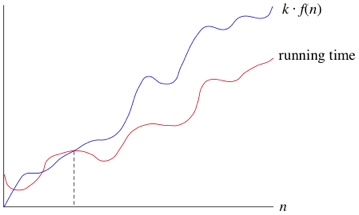
\includegraphics[width=0.3\textwidth]{figure_man/bigo.png}~~
  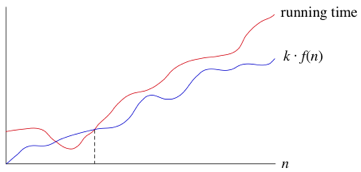
\includegraphics[width = 0.3\textwidth]{figure_man/bigomega.png}~~
  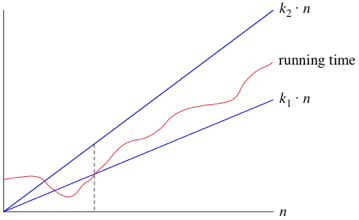
\includegraphics[width = 0.3\textwidth]{figure_man/bigtheta.png} \\
  %\caption{$O(f(n))$, $\Omega(f(n))$ and $\Theta(f(n))$}
\end{figure}
\end{center}

Left panel $O(f(n))$, middle panel $\Omega(f(n))$ and right panel $\Theta(f(n))$


\end{vbframe}

\begin{vbframe}{Complexity vs. empirical runtime}

In this chapter we dealt with the \textbf{complexity of algorithms}:

\begin{itemize}
\item How does an algorithm \textbf{scale} with regards to the required resources?
\item What happens when the problem gets bigger?
\item What is the theoretical runtime complexity of an algorithm? (Knowledge / Estimation / Evidence)
\begin{itemize}
\item Bubble sort has a worst-case runtime of $\order(n^2)$
\item Matrix multiplication of two regular $n\times n$ matrices has a runtime complexity of $\order(n^3)$
\item The Traveling Salesman Problem is NP-complete
\item ...
\end{itemize}
\item It is often helpful to test the complexity of an algorithm empirically!
\end{itemize}

\framebreak

\textbf{But:} How many resources does my algorithm \textbf{really} need?\\
$\to$ \textbf{empirical runtime analysis}:

\begin{itemize}
\item Measurement of the runtime of an implementation on a given machine
\item How much time (or memory etc.) is needed when the code is executed?
\item $\to$ Depends on the machine, the compiler/interpreter, dependencies, and the code itself
\item The empirical runtime can be measured for a fixed input quantity, but can also be systematically analyzed for different input quantities / problem instances
\item When computing on a cluster, the cloud, or a machine on which several people are computing, the empirical run-time is usually influenced by the actions of other users
\end{itemize}

\end{vbframe}

\endlecture
\end{document}

